\documentclass[UTF8,zihao=-4,scheme=chinese,fontset=none]{ctexart}
\usepackage[a4paper,top=2.5cm,bottom=2.5cm,left=2.8cm,right=2.8cm,headheight=15pt]{geometry}
\usepackage{fontspec,xeCJK,setspace,indentfirst,fancyhdr,booktabs,tabularx,array,longtable,graphicx,float,caption,listings,xcolor,enumitem,amsmath,url}
\usepackage{unicode-math}
\usepackage{tikz}
\usetikzlibrary{arrows.meta,positioning,shapes.geometric}
\usepackage[hidelinks,unicode]{hyperref}

\IfFileExists{fonts/times.ttf}{\setmainfont[Path=fonts/,BoldFont=timesbd.ttf,ItalicFont=timesi.ttf,BoldItalicFont=timesbi.ttf]{times.ttf}}{\setmainfont{TeX Gyre Termes}}
\IfFileExists{fonts/simsun.ttc}{\setCJKmainfont[Path=fonts/]{simsun.ttc}}{\setCJKmainfont{FandolSong-Regular}}
\IfFileExists{fonts/times.ttf}{\setmonofont[Path=fonts/]{times.ttf}}{}
\IfFileExists{fonts/times.ttf}{\setsansfont[Path=fonts/,BoldFont=timesbd.ttf,ItalicFont=timesi.ttf,BoldItalicFont=timesbi.ttf]{times.ttf}}{}
\IfFileExists{fonts/simsun.ttc}{\setCJKmonofont[Path=fonts/]{simsun.ttc}}{}
\IfFileExists{fonts/cambria.ttc}{\setmathfont[Path=fonts/,FontIndex=1]{cambria.ttc}}{}

\setlength{\parindent}{2em}
\setlength{\parskip}{0pt}
\linespread{1.35}
\setlength{\emergencystretch}{2em}
\renewcommand{\arraystretch}{1.22}
\setlist{nosep,leftmargin=2em}
\setcounter{tocdepth}{2}
\graphicspath{{figures/}}

\ctexset{
  section={format=\bfseries\zihao{3},name={Chapter\space,},number=\arabic{section},beforeskip=.8em,afterskip=.7em},
  subsection={format=\bfseries\zihao{4},beforeskip=.7em,afterskip=.4em},
  subsubsection={format=\bfseries\zihao{-4}}
}
\captionsetup{font=small,labelsep=quad,labelfont=bf}
\renewcommand{\contentsname}{Contents}
\renewcommand{\refname}{References}
\renewcommand{\figurename}{Figure}
\renewcommand{\tablename}{Table}

\pagestyle{fancy}
\fancyhf{}
\fancyhead[C]{\zihao{5}Experiment 2 Individual Report: Fixed-Point Pick-and-Place}
\fancyfoot[C]{\thepage}
\renewcommand{\headrulewidth}{.4pt}

\definecolor{codegray}{gray}{.95}
\definecolor{darkblue}{RGB}{25,70,135}
\definecolor{darkgreen}{RGB}{0,105,60}
\definecolor{darkorange}{RGB}{175,85,0}
\definecolor{darkred}{RGB}{145,25,25}
\definecolor{lightblue}{RGB}{232,241,252}
\lstset{
  basicstyle=\ttfamily\zihao{5},
  backgroundcolor=\color{codegray},
  frame=single,
  rulecolor=\color{black},
  breaklines=true,
  columns=fullflexible,
  keepspaces=true,
  showstringspaces=false,
  numbers=left,
  numberstyle=\tiny,
  xleftmargin=2em,
  framexleftmargin=1.5em
}
\newcolumntype{Y}{>{\raggedright\arraybackslash}X}
\newcommand{\completed}{\textcolor{darkgreen}{\textbf{Completed}}}
\newcommand{\evidence}{\textcolor{darkblue}{\textbf{Verified evidence}}}
\newcommand{\githuburl}{\url{https://github.com/xhr-CHN/mecharm-fixed-point-pick-place}}

\begin{document}

\begin{titlepage}
\thispagestyle{empty}
\begin{center}
\vspace*{1.6cm}
{\bfseries\zihao{1}Experiment 2: Fixed-Point Robotic-Arm Pick-and-Place\par}
\vspace{.7cm}
{\bfseries\zihao{2}Individual Experimental Report\par}
\vspace{.35cm}
{\bfseries\zihao{3}Isaac Sim mechArm Simulation and DJI RoboMaster EP Verification\par}
\vspace{2.0cm}
\renewcommand{\arraystretch}{1.9}
\begin{tabular}{>{\bfseries}p{3.3cm}p{8.0cm}}
Course: & Robotic Systems Integration Laboratory\\
Experiment: & Fixed-Point Robotic-Arm Pick-and-Place\\
Report Type: & Individual Report\\
Name: & Haoran Xiao\\
Student ID: & 24020036066\\
Project Role: & Simulation, control integration, debugging, physical verification, and documentation\\
GitHub: & \href{https://github.com/xhr-CHN/mecharm-fixed-point-pick-place}{xhr-CHN/mecharm-fixed-point-pick-place}\\
Period: & August 31--September 9, 2026\\
\end{tabular}
\vfill
{\bfseries\zihao{3}September 9, 2026\par}
\end{center}
\end{titlepage}

\pagenumbering{Roman}
\setcounter{page}{1}

\section*{Abstract}
\addcontentsline{toc}{section}{Abstract}
This individual report describes my work on Experiment 2, a fixed-point robotic pick-and-place task completed in both simulation and on a physical robot. The available platforms were different, so I used a mechArm 270 Pi with an adaptive gripper in Isaac Sim 5.1.0 for the simulation stage and a DJI RoboMaster EP for the physical stage. In simulation, I built the scene, integrated the official Elephant Robotics model, connected Windows Isaac Sim to ROS 2 Humble in Docker through a TCP bridge, implemented numerical inverse kinematics and smooth direct joint execution, repaired the adaptive gripper's missing closed-loop pin constraints, and completed a five-cycle alternating transfer between two fixed points. For physical verification, I implemented and tested a five-cycle RoboMaster EP program with arm motion, chassis rotation, gripper-state feedback, automatic retry, camera monitoring, and a safe-exit key.

The project required substantial diagnosis across robot modeling, middleware discovery, container networking, trajectory generation, inverse-kinematics reachability, and contact dynamics. I therefore focus not only on the final workflow but also on the reasoning that connected each symptom to its root cause. Public GitHub evidence contains 31 pushed project commits authored by my account, while the local branch contains two additional report-planning commits. Simulation and physical recordings preserve both successful repeated operation and failure behavior. The final result demonstrates a reproducible fixed-point manipulation workflow and, more importantly, a systematic method for integrating software, simulation physics, and real hardware.

\noindent\textbf{Keywords:} fixed-point grasping; mechArm 270 Pi; Isaac Sim; ROS 2 Humble; inverse kinematics; adaptive gripper; RoboMaster EP; trajectory smoothing

\clearpage
\begingroup\zihao{5}\linespread{.92}\selectfont
\tableofcontents
\endgroup
\clearpage

\pagenumbering{arabic}
\setcounter{page}{1}

\section{Basic Experimental Requirements}

\subsection{Experimental Objective}

The experiment required a robot to transfer an object between two known locations without visual localization. Because both points were predetermined, the essential engineering problem was not object detection but reliable motion execution: the robot had to start from a safe HOME posture, approach the object, align the gripper, close it without collision, lift the object, move to the destination, release it, and return safely.

I summarized the required state sequence as
\begin{equation}
\mathrm{HOME}\rightarrow\mathrm{PREGRASP}\rightarrow\mathrm{DESCEND}\rightarrow
\mathrm{CLOSE}\rightarrow\mathrm{LIFT}\rightarrow\mathrm{PLACE}\rightarrow
\mathrm{OPEN}\rightarrow\mathrm{HOME}.
\end{equation}
The experiment also required repeated execution, visible state or error information, and safe behavior when a target was unreachable or a grasp failed.

\subsection{Platforms Used in the Completed Experiment}

The available equipment determined the implementation platform for each stage. I completed the simulation using the mechArm 270 Pi model and completed the physical stage using a DJI RoboMaster EP. This was a practical platform adaptation rather than an incomplete substitution: the two platforms demonstrated the same manipulation concept through their own suitable motion interfaces.

\begin{table}[H]
\centering
\caption{Completed experiment stages and platforms}
\begin{tabularx}{\textwidth}{p{2.9cm}p{3.8cm}Yp{2.1cm}}
\toprule
Stage & Platform & Main verification target & Status\\
\midrule
Simulation & mechArm 270 Pi adaptive-gripper model in Isaac Sim 5.1.0 & Cartesian approach, vertical grasp, A/B transfer, five alternating cycles, exceptions, and physics stability & \completed\\
Physical robot & DJI RoboMaster EP with robotic arm, gripper, chassis, and camera & Real grasp, transport through chassis rotation, release, automatic retry, safe exit, and five successful cycles & \completed\\
\bottomrule
\end{tabularx}
\end{table}

The simulation host was Windows, while ROS 2 Humble and MoveIt 2 ran in a dedicated Ubuntu 22.04 Docker image. Isaac Sim and the container exchanged commands and measured joint states through a project-specific TCP bridge on port 8765. The physical RoboMaster program ran from Windows with the official RoboMaster Python SDK and connected to the robot in AP mode over TCP.

\subsection{Functional and Safety Requirements}

I translated the basic requirements into testable engineering items before implementation. The resulting checklist is shown in Table~\ref{tab:reqmatrix}.

\begin{longtable}{p{4.0cm}p{7.1cm}p{2.0cm}}
\caption{Requirement-to-evidence matrix}\label{tab:reqmatrix}\\
\toprule Requirement & Implemented evidence & Result\\
\midrule\endfirsthead
\toprule Requirement & Implemented evidence & Result\\
\midrule\endhead
Known pick and place locations & Parameterized A and B coordinates in the ROS 2 Cartesian configuration & \completed\\
Safe initial state & Defined HOME pose; every simulation cycle and every physical attempt begins and ends in a safe posture & \completed\\
Complete pick-and-place sequence & Open, approach, descend, close, lift, transfer, release, retreat, and HOME & \completed\\
Vertical grasp in simulation & Tool-axis constraint and a grasp-phase yaw offset used consistently through grasp and transport & \completed\\
Repeated operation & Five alternating A-to-B/B-to-A simulation cycles and five successful RoboMaster EP physical cycles & \completed\\
Failure handling & IK rejection, stale-feedback timeout, empty-grasp test, RoboMaster unknown-state timeout, retry, and safe exit & \completed\\
Observable evidence & GitHub history, terminal logs, simulation recordings, a failure recording, and a physical recording & \completed\\
Reproducible startup & PowerShell, Docker Compose, ROS 2 launch, scene rebuild, and physical SDK commands documented & \completed\\
\bottomrule
\end{longtable}

\subsection{Evaluation Criteria I Used}

I considered the experiment successful only when the following conditions were visible together:
\begin{enumerate}
\item the robot started from a predictable HOME or parked posture;
\item the end effector reached a collision-free position above the target;
\item the gripper orientation and closing height matched the object's geometry;
\item the object was lifted before horizontal transport;
\item the object was released at the opposite point;
\item the robot returned to its initial posture before the next cycle;
\item failures produced a clear message and a bounded recovery rather than uncontrolled motion.
\end{enumerate}
These criteria shaped both my code structure and my debugging decisions.

\section{Individual Responsibilities and Contributions}

\subsection{Scope of My Work}

My work covered the full path from an empty repository structure to recorded simulation and physical-robot demonstrations. I organized the workspace, created the public repository, integrated the model, implemented the control programs, diagnosed middleware and physics failures, tuned the task parameters, wrote the startup documentation, recorded the experiments, and prepared the final reports.

I did not treat these as unrelated tasks. For example, a gripper-model defect directly changed the feasible trajectory and contact behavior; network discovery affected whether RViz and MoveIt appeared functional; and the hardware platform changed the available feedback signal for grasp detection. My responsibility was therefore system integration across these boundaries.

\subsection{Git History as Verifiable Evidence}

At the time of evidence capture, the public \texttt{origin/main} branch contained 31 commits, all authored by the GitHub account \texttt{xhr-CHN}. The local \texttt{main} branch contained 33 commits because it also included the individual-report design and implementation-plan commits. Figure~\ref{fig:github} is a direct screenshot of the public GitHub commit page. It shows a representative continuous sequence of my feature, fix, tuning, and documentation commits.

\begin{figure}[H]
\centering
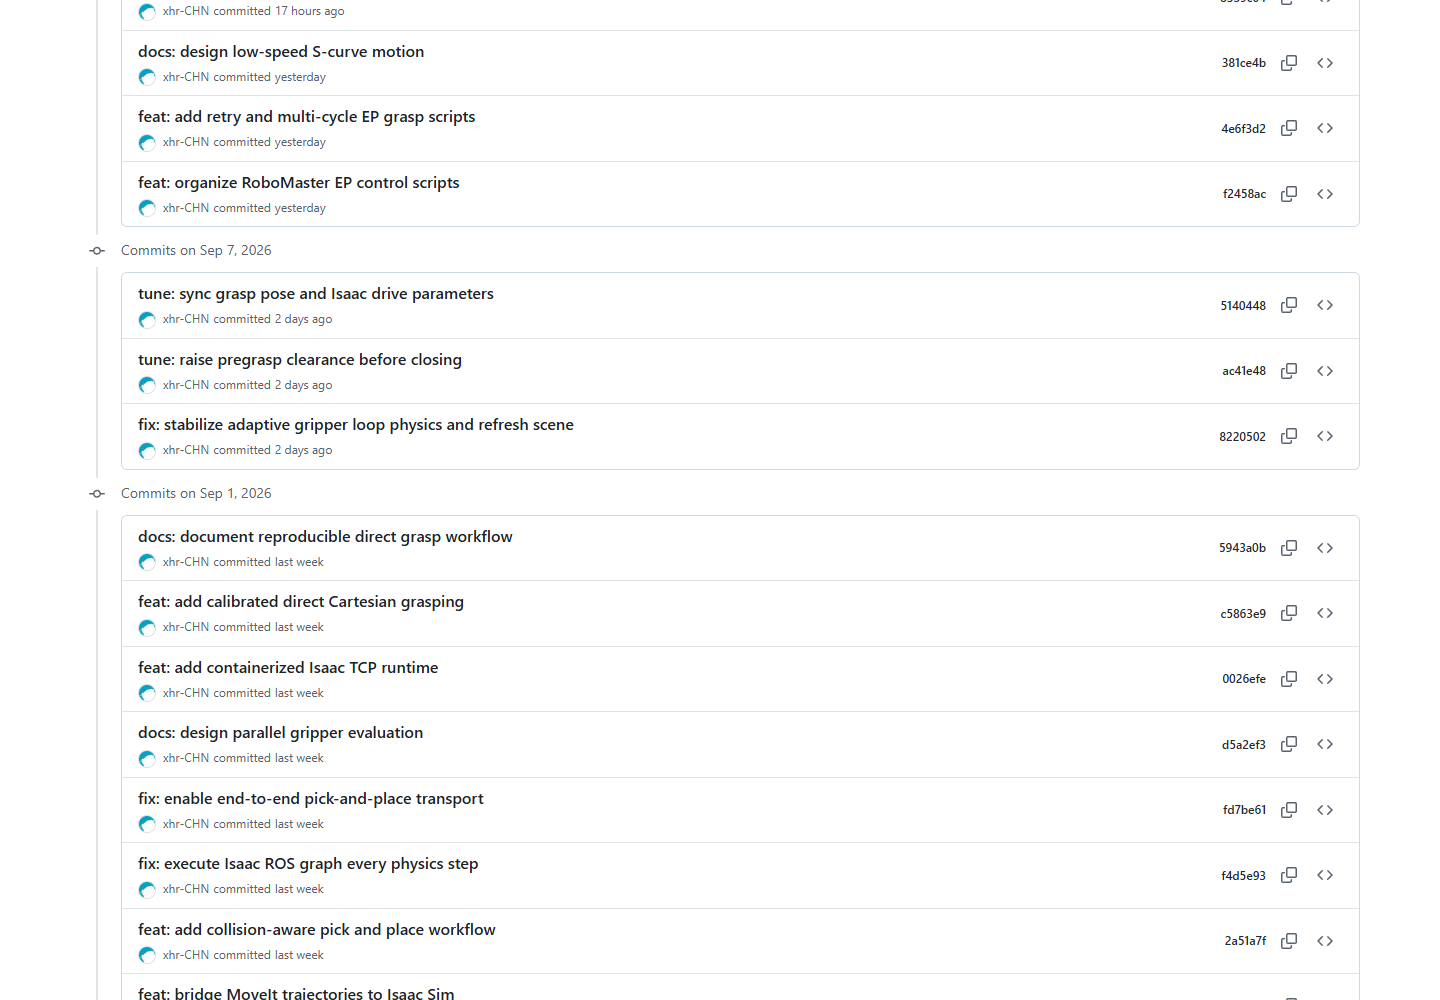
\includegraphics[width=.96\textwidth]{github_commit_history.png}
\caption{Public GitHub commit-history excerpt showing implementation, repair, tuning, and documentation commits authored by \texttt{xhr-CHN}}
\label{fig:github}
\end{figure}

I use this history only as evidence of my own sustained work. The strongest contribution evidence is the combination of commit history, corresponding source files, runtime logs, and recorded behavior.

\subsection{My Contribution Breakdown}

\begingroup\small
\begin{longtable}{p{2.9cm}p{7.1cm}p{2.9cm}}
\caption{Personal contribution breakdown}\label{tab:contrib}\\
\toprule Area & Work I completed & Representative evidence\\
\midrule\endfirsthead
\toprule Area & Work I completed & Representative evidence\\
\midrule\endhead
Repository engineering & Created the repository structure, staged commits in logical increments, maintained \texttt{main}, added bilingual README files, and organized large videos with Git LFS & Git history and README files\\
Robot model & Integrated Elephant Robotics mechArm 270 Pi and adaptive-gripper URDF/meshes, generated the USD scene, and retained the source license & \texttt{simulation/urdf/} and USD scene\\
Simulation scene & Added table, block, lighting, camera, fixed points, safe height, articulation setup, physics step, and render settings & Figure~\ref{fig:scene} and scene generator\\
ROS 2 integration & Built ROS 2 packages, MoveIt configuration, task nodes, launch files, state publishing, and trajectory interfaces & \texttt{src/} packages and launch files\\
Cross-system transport & Replaced unreliable cross-OS DDS discovery with a narrow TCP bridge carrying joint state and targets & Port 8765 bridge and probe logs\\
Kinematics & Implemented numerical IK with position, finite-value, joint-limit, and vertical-axis checks & \texttt{numeric\_ik.py}\\
Motion quality & Implemented quintic interpolation, 120 Hz target streaming, separate normal/vertical speed limits, feedback pacing, and timeout handling & Direct motion programs\\
Gripper mechanics & Diagnosed missing closed-loop pins, repaired the two distal loop constraints, added visible pins, disabled unreliable mimic parsing, and mirrored inner-joint commands & Figures~\ref{fig:holes} and~\ref{fig:pins}\\
Repeated simulation & Implemented A-to-B/B-to-A alternation for five cycles, returning HOME after every transfer & Figure~\ref{fig:simfive}\\
Exception behavior & Implemented unreachable-IK rejection, stale-feedback timeout, and an intentional empty-grasp test with HOME recovery & Failure recording and logs\\
Physical verification & Implemented connection tests, small-motion tests, one-cycle and five-cycle EP programs, camera display, feedback-based grasp inference, retry, and E-key safe exit & Figure~\ref{fig:hardware}\\
Documentation & Wrote Chinese and English instructions, model source notes, test records, and experiment reports & \texttt{README.md}, \texttt{README\_EN.md}, \texttt{docs/}, and \texttt{report/}\\
\bottomrule
\end{longtable}
\endgroup

\subsection{Development Timeline}

My commit history also records how the system evolved:
\begin{itemize}
\item \textbf{August 31:} repository structure, experiment overview, simulation configuration, ROS 2 package metadata, Isaac integration, model assets, and the first smooth in-app demonstration;
\item \textbf{September 1:} MoveIt configuration, trajectory bridge, collision-aware workflow, Isaac graph stepping, end-to-end transport repair, and containerized TCP runtime;
\item \textbf{September 2:} calibrated Cartesian grasping and reproducible direct-grasp documentation;
\item \textbf{September 7:} adaptive-gripper loop repair, pre-grasp clearance correction, pose calibration, and drive-parameter synchronization;
\item \textbf{September 8:} RoboMaster EP programs, retry logic, five-cycle recordings, and bilingual final documentation;
\item \textbf{September 9:} evidence-driven individual report design, implementation, and verification.
\end{itemize}
This sequence shows that I first established basic movement, then solved integration and physical-model defects, and only then finalized repeated operation and documentation.

\section{Principles and Project Implementation}

\subsection{Overall System Architecture}

The main simulation challenge was that Isaac Sim ran natively on Windows while ROS 2 and MoveIt ran in Docker. I separated planning/control from physics, with the TCP bridge as a narrow transport boundary.

\begin{figure}[H]
\centering
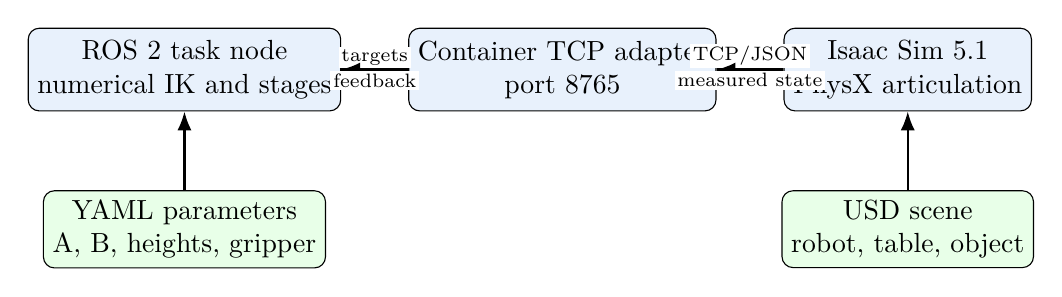
\begin{tikzpicture}[
  node distance=1.0cm and .85cm,
  block/.style={draw,rounded corners,minimum width=2.75cm,minimum height=1.05cm,align=center,fill=lightblue},
  data/.style={draw,rounded corners,minimum width=2.6cm,minimum height=.85cm,align=center,fill=green!9},
  arrow/.style={-{Latex[length=2.4mm]},thick}
]
\node[block] (task) {ROS 2 task node\\numerical IK and stages};
\node[block,right=of task] (bridge) {Container TCP adapter\\port 8765};
\node[block,right=of bridge] (isaac) {Isaac Sim 5.1\\PhysX articulation};
\node[data,below=of task] (yaml) {YAML parameters\\A, B, heights, gripper};
\node[data,below=of isaac] (usd) {USD scene\\robot, table, object};
\draw[arrow] (yaml)--(task);
\draw[arrow] (task)--node[above,fill=white,inner sep=1pt,font=\scriptsize]{targets}(bridge);
\draw[arrow] (bridge)--node[above,fill=white,inner sep=1pt,font=\scriptsize]{TCP/JSON}(isaac);
\draw[arrow] (isaac)--node[below,fill=white,inner sep=1pt,font=\scriptsize]{measured state}(bridge);
\draw[arrow] (bridge)--node[below,fill=white,inner sep=1pt,font=\scriptsize]{feedback}(task);
\draw[arrow] (usd)--(isaac);
\end{tikzpicture}
\caption{Simulation control architecture implemented for Experiment 2}
\label{fig:architecture}
\end{figure}

This architecture kept the ROS graph container-local and removed the need for DDS multicast to cross Windows, WSL, Docker, and proxy/TUN boundaries. The transport sent only the state needed by this experiment, which made failures easier to isolate.

\subsection{Scene and Official Robot Model}

I based the robot description on the Humble branch of Elephant Robotics' official \texttt{mycobot\_ros2} repository\cite{elephantrepo}. The imported assets include the mechArm 270 Pi arm and adaptive gripper meshes. The experiment scene contains a fixed-base robot, table, target block, camera, lights, and configured pick/place locations.

\begin{figure}[H]
\centering
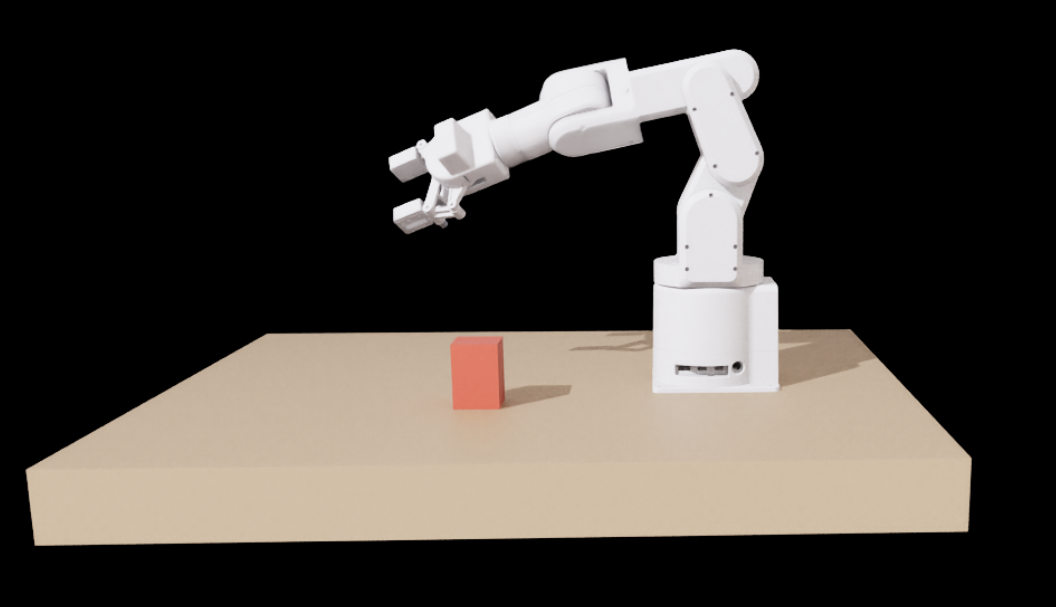
\includegraphics[width=.90\textwidth]{isaac_scene.png}
\caption{Completed Isaac Sim scene with mechArm 270 Pi, table, adaptive gripper, and target block}
\label{fig:scene}
\end{figure}

The physics world runs at 120 Hz and renders at 60 Hz. The checked-in scene generator imports the arm with default drive strength 1000 and damping 30000. The adaptive-gripper driven joints are then tuned separately to stiffness 150, damping 60, and maximum force 10. This separation was important because arm holding strength and closed-loop gripper stability require different drive behavior.

\subsection{Fixed Cartesian Targets}

The final simulation parameters were
\begin{align}
\mathbf{p}_{A} &= (0.18,\ 0.09,\ 0.025)\ \mathrm{m},\\
\mathbf{p}_{B} &= (0.18,\ -0.08,\ 0.025)\ \mathrm{m}.
\end{align}
The pre-grasp clearance is 0.10 m, so the first Cartesian target above the object is at approximately $z=0.125$ m. The closing clearance is 0.04 m, giving a closing target at approximately $z=0.065$ m. Since the top of the block is near $z=0.050$ m, the fingers can surround the block without the palm colliding with it before closure.

The HOME joint pose is
\begin{equation}
\mathbf{q}_{\mathrm{home}}=(0,0,0,-47,0,0)^{\circ}.
\end{equation}
Every cycle returns to this pose before the next cycle starts.

\subsection{Numerical Inverse Kinematics and Grasp Orientation}

The numerical IK solver parses the same URDF that defines the simulated robot. For a candidate joint vector $\mathbf{q}$, forward kinematics produces the tool position $\mathbf{p}(\mathbf{q})$ and tool axis $\mathbf{a}(\mathbf{q})$. I accepted a solution only when
\begin{align}
\left\|\mathbf{p}(\mathbf{q})-\mathbf{p}_{d}\right\| &\leq 0.008\ \mathrm{m},\\
\mathbf{a}(\mathbf{q})\cdot\mathbf{a}_{d} &\geq 0.975,
\end{align}
and all joint values were finite and within URDF limits.

The end effector also uses a $90^{\circ}$ yaw offset relative to the HOME tool direction during the grasp phase. A key design decision was to carry the same orientation through pre-grasp, descent, lift, transport, placement, and retreat. Changing the yaw only at one waypoint would create unnecessary wrist motion and could turn a valid grasp into a collision.

\subsection{Smooth Joint Execution}

The first direct commands caused visible jerk and excited the compliant dynamics. I replaced piecewise target jumps with a quintic smoothstep:
\begin{equation}
s(u)=6u^{5}-15u^{4}+10u^{3},\qquad 0\leq u\leq1,
\end{equation}
\begin{equation}
\mathbf{q}(u)=\mathbf{q}_{0}+s(u)(\mathbf{q}_{1}-\mathbf{q}_{0}).
\end{equation}
This polynomial has zero velocity and zero acceleration at both endpoints. Targets are streamed at 120 Hz and paced using measured feedback. If valid feedback is absent for more than 5 s, the program stops the segment instead of continuing open-loop.

I used two speed limits because vertical contact motion needs more control than free-space transit:
\begin{itemize}
\item normal arm stages: $28^{\circ}/\mathrm{s}$ maximum peak joint speed;
\item vertical descent/lift stages: $4^{\circ}/\mathrm{s}$ maximum peak joint speed;
\item adaptive-gripper command: $0.12\ \mathrm{rad}/\mathrm{s}$ with 1.0 s pre-command and 1.5 s post-command waits.
\end{itemize}
This preserved reasonable cycle time while keeping the grasp approach slow.

\subsection{Adaptive-Gripper Four-Bar Repair}

The adaptive gripper was the most important model-level problem. The official URDF is a tree, but the real gripper contains closed four-bar linkages. Two distal pin joints that physically connect the inner and outer links are therefore not expressible as ordinary URDF tree joints. The imported model visually contained pivot holes but lacked the two physical loop closures.

\begin{figure}[H]
\centering
\begin{minipage}{.48\textwidth}
\centering
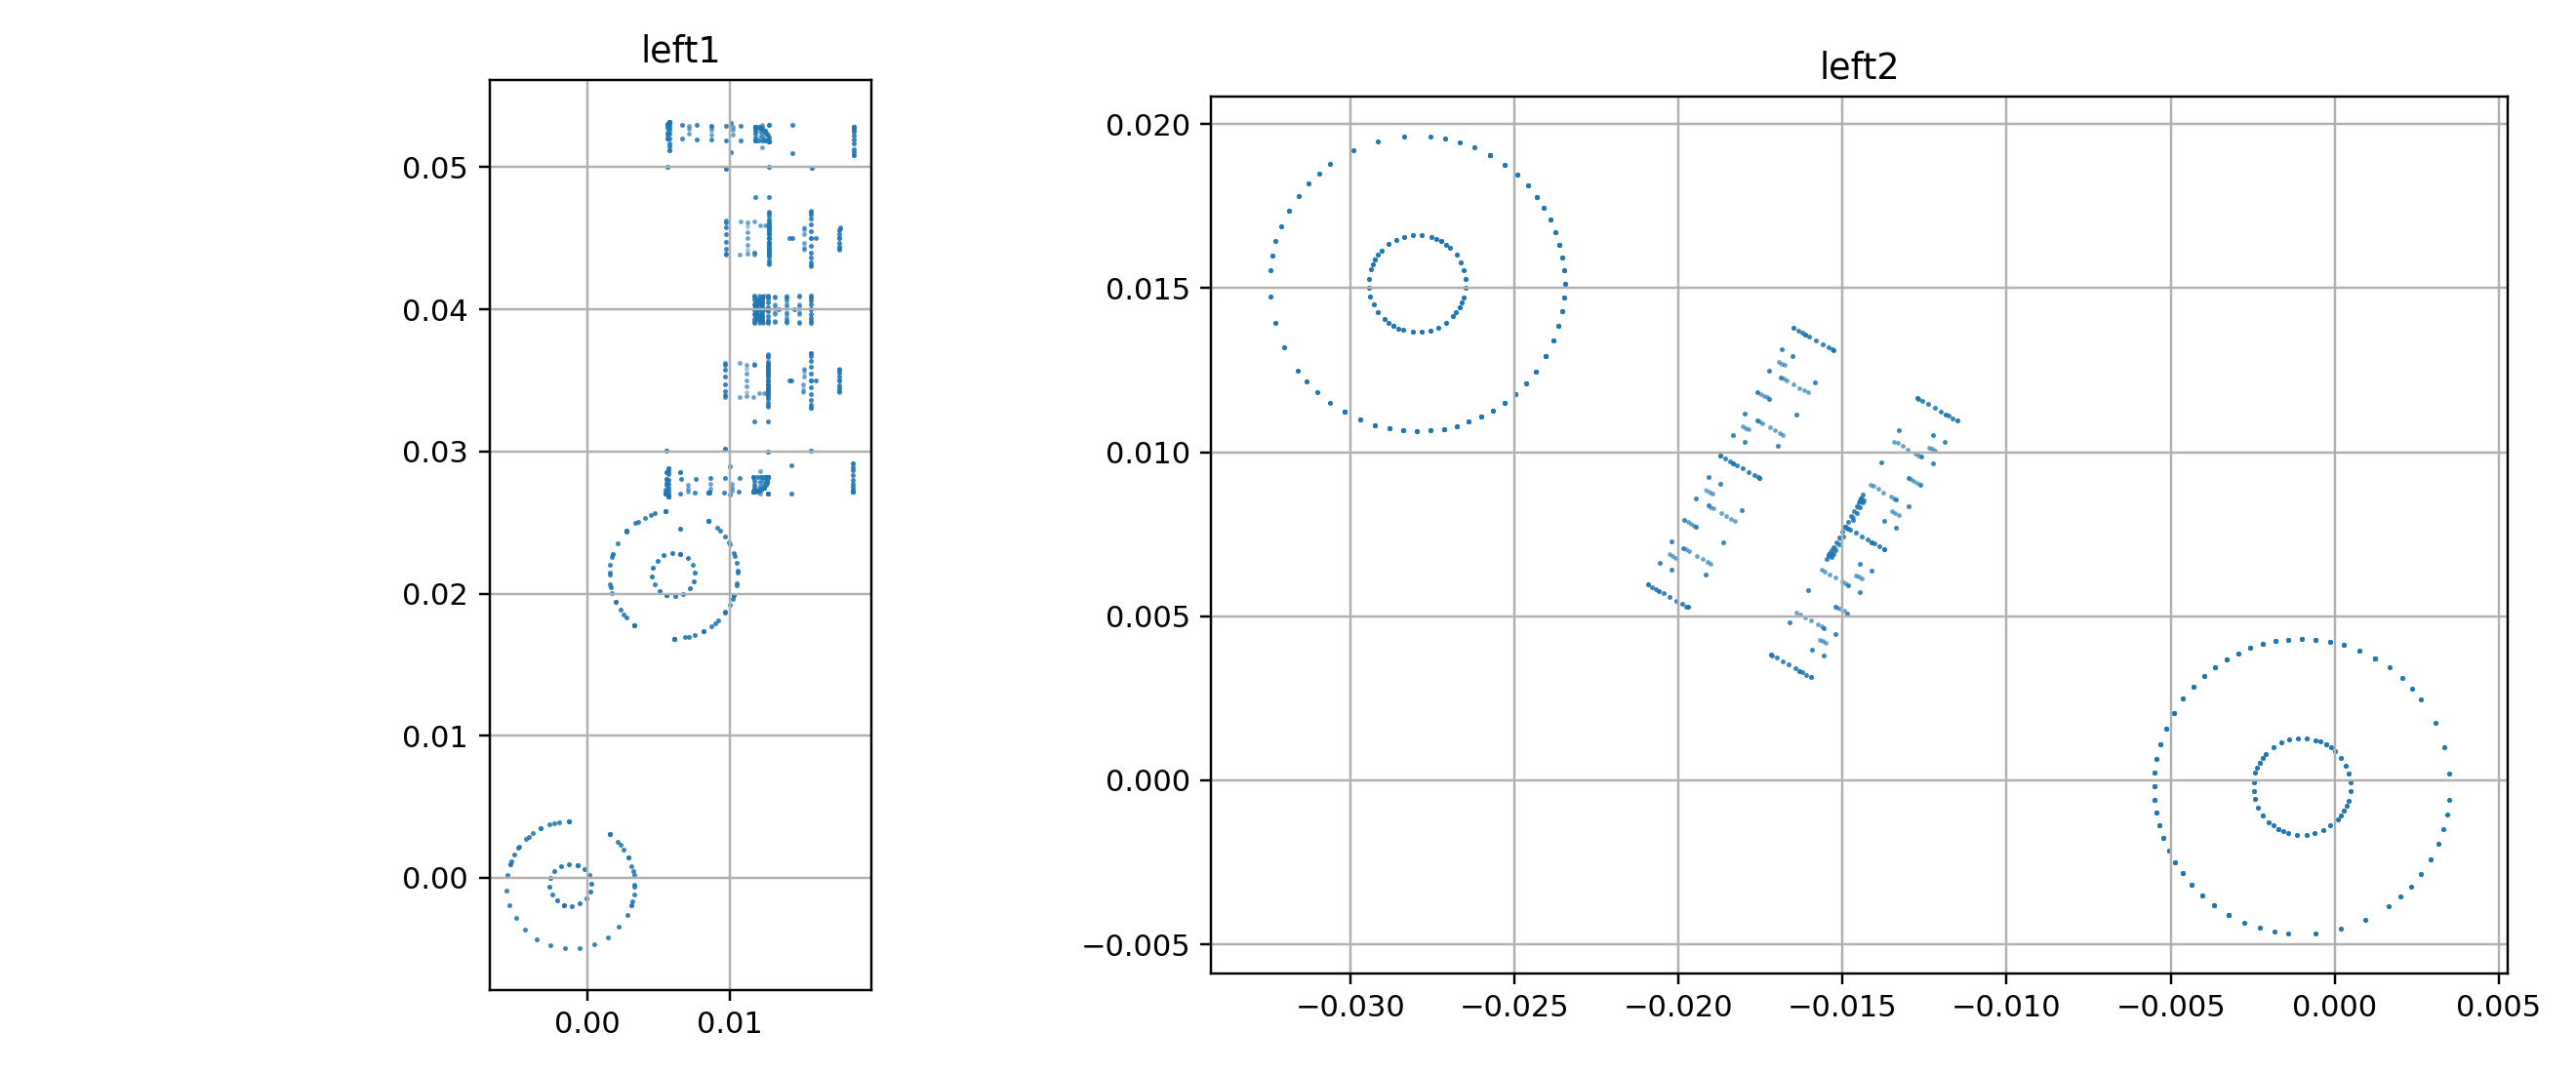
\includegraphics[width=\textwidth]{gripper_hole_projection_scene.png}
\caption*{(a) Projected locations of the missing loop closures}
\end{minipage}\hfill
\begin{minipage}{.48\textwidth}
\centering
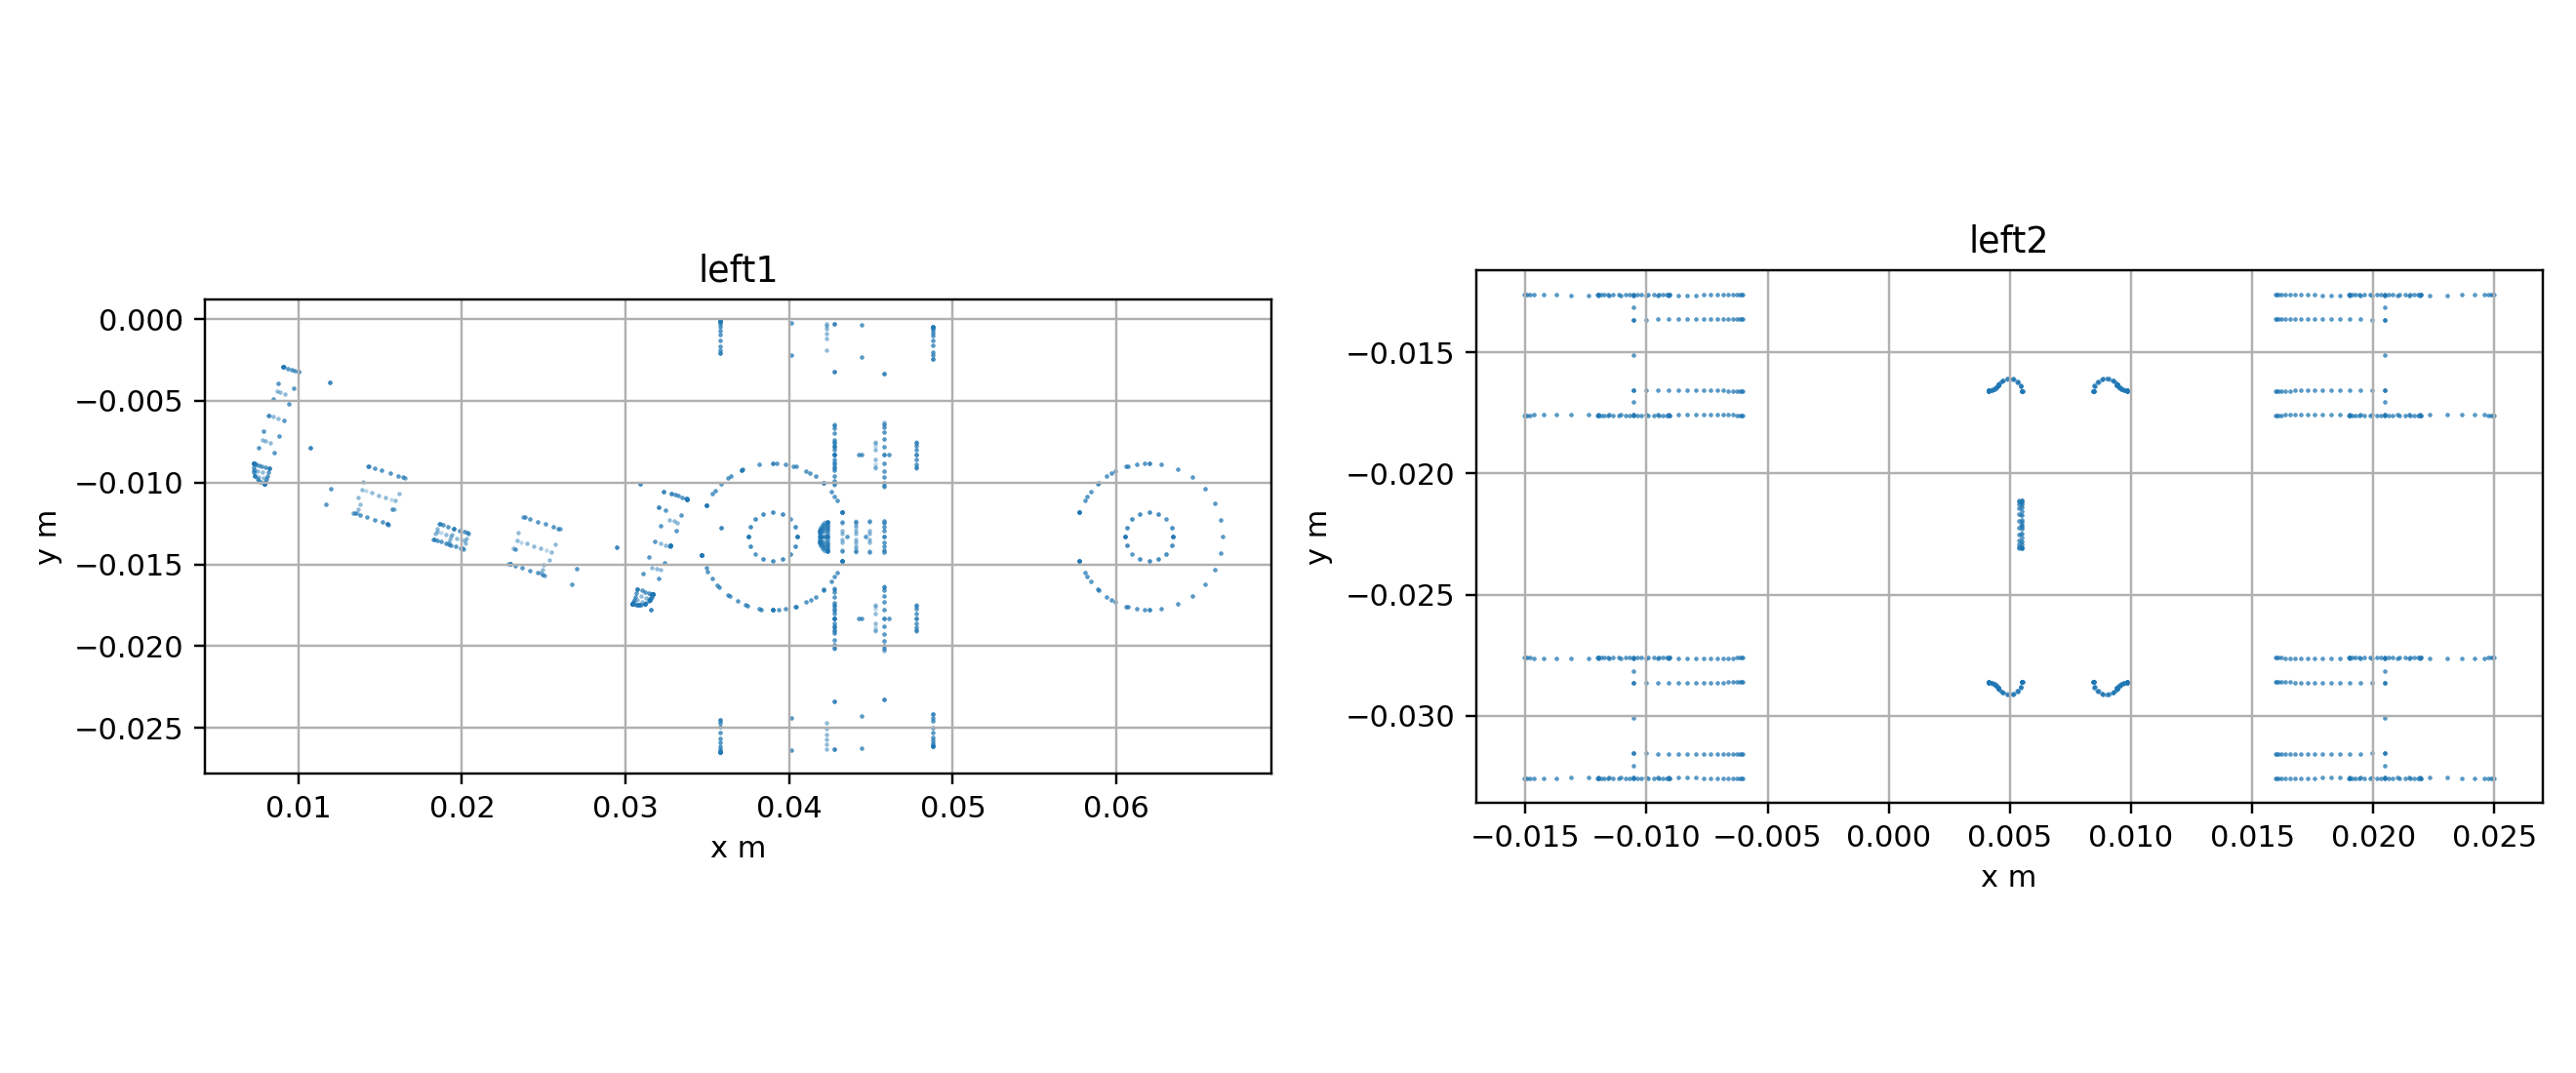
\includegraphics[width=\textwidth]{gripper_hole_projection.png}
\caption*{(b) Linkage geometry used to align the pivots}
\end{minipage}
\caption{Geometric diagnosis of the adaptive-gripper linkage}
\label{fig:holes}
\end{figure}

I repaired the mechanism in four steps:
\begin{enumerate}
\item disabled URDF mimic parsing because PhysX 5.1 did not reliably support multiple followers of the same reference joint;
\item added explicit angular drives to the inner links and mirrored the master command in the TCP joint bridge;
\item made the outer jaws passive and added two PhysX revolute loop joints between the inner and outer distal links;
\item added four visible, non-colliding cylinder pins so the physical constraints also had a clear visual representation.
\end{enumerate}
The mirrored command relationship is
\begin{equation}
q_{L}=q_{m},\qquad q_{R2}=q_{R3}=-q_{m},
\end{equation}
while the passive outer jaws follow through the loop constraints. The scene uses 64 position and 64 velocity solver iterations and selective self-collision to improve stability.

\begin{figure}[H]
\centering
\fbox{\begin{minipage}{.88\textwidth}
\small
\textbf{Implemented pin model.} The scene generator creates two excluded-from-articulation PhysX revolute joints named \texttt{gripper\_left\_loop\_joint} and \texttt{gripper\_right\_loop\_joint}. Four visible pins are placed at the base and distal pivots. The distal pair closes the two four-bar loops; the base pair represents the already constrained pivots. Pin meshes are visual only and do not create duplicate collisions.
\end{minipage}}
\caption{Logical structure of the repaired gripper constraints}
\label{fig:pins}
\end{figure}

\subsection{Five-Cycle Alternating Simulation}

The repeated task alternates the source and destination:
\begin{equation}
A\rightarrow B,\quad B\rightarrow A,\quad A\rightarrow B,\quad B\rightarrow A,\quad A\rightarrow B.
\end{equation}
After each placement, the robot returns HOME before beginning the next grasp. This makes each cycle independently observable and prevents pose drift from being hidden inside a long uninterrupted trajectory.

\begin{figure}[H]
\centering
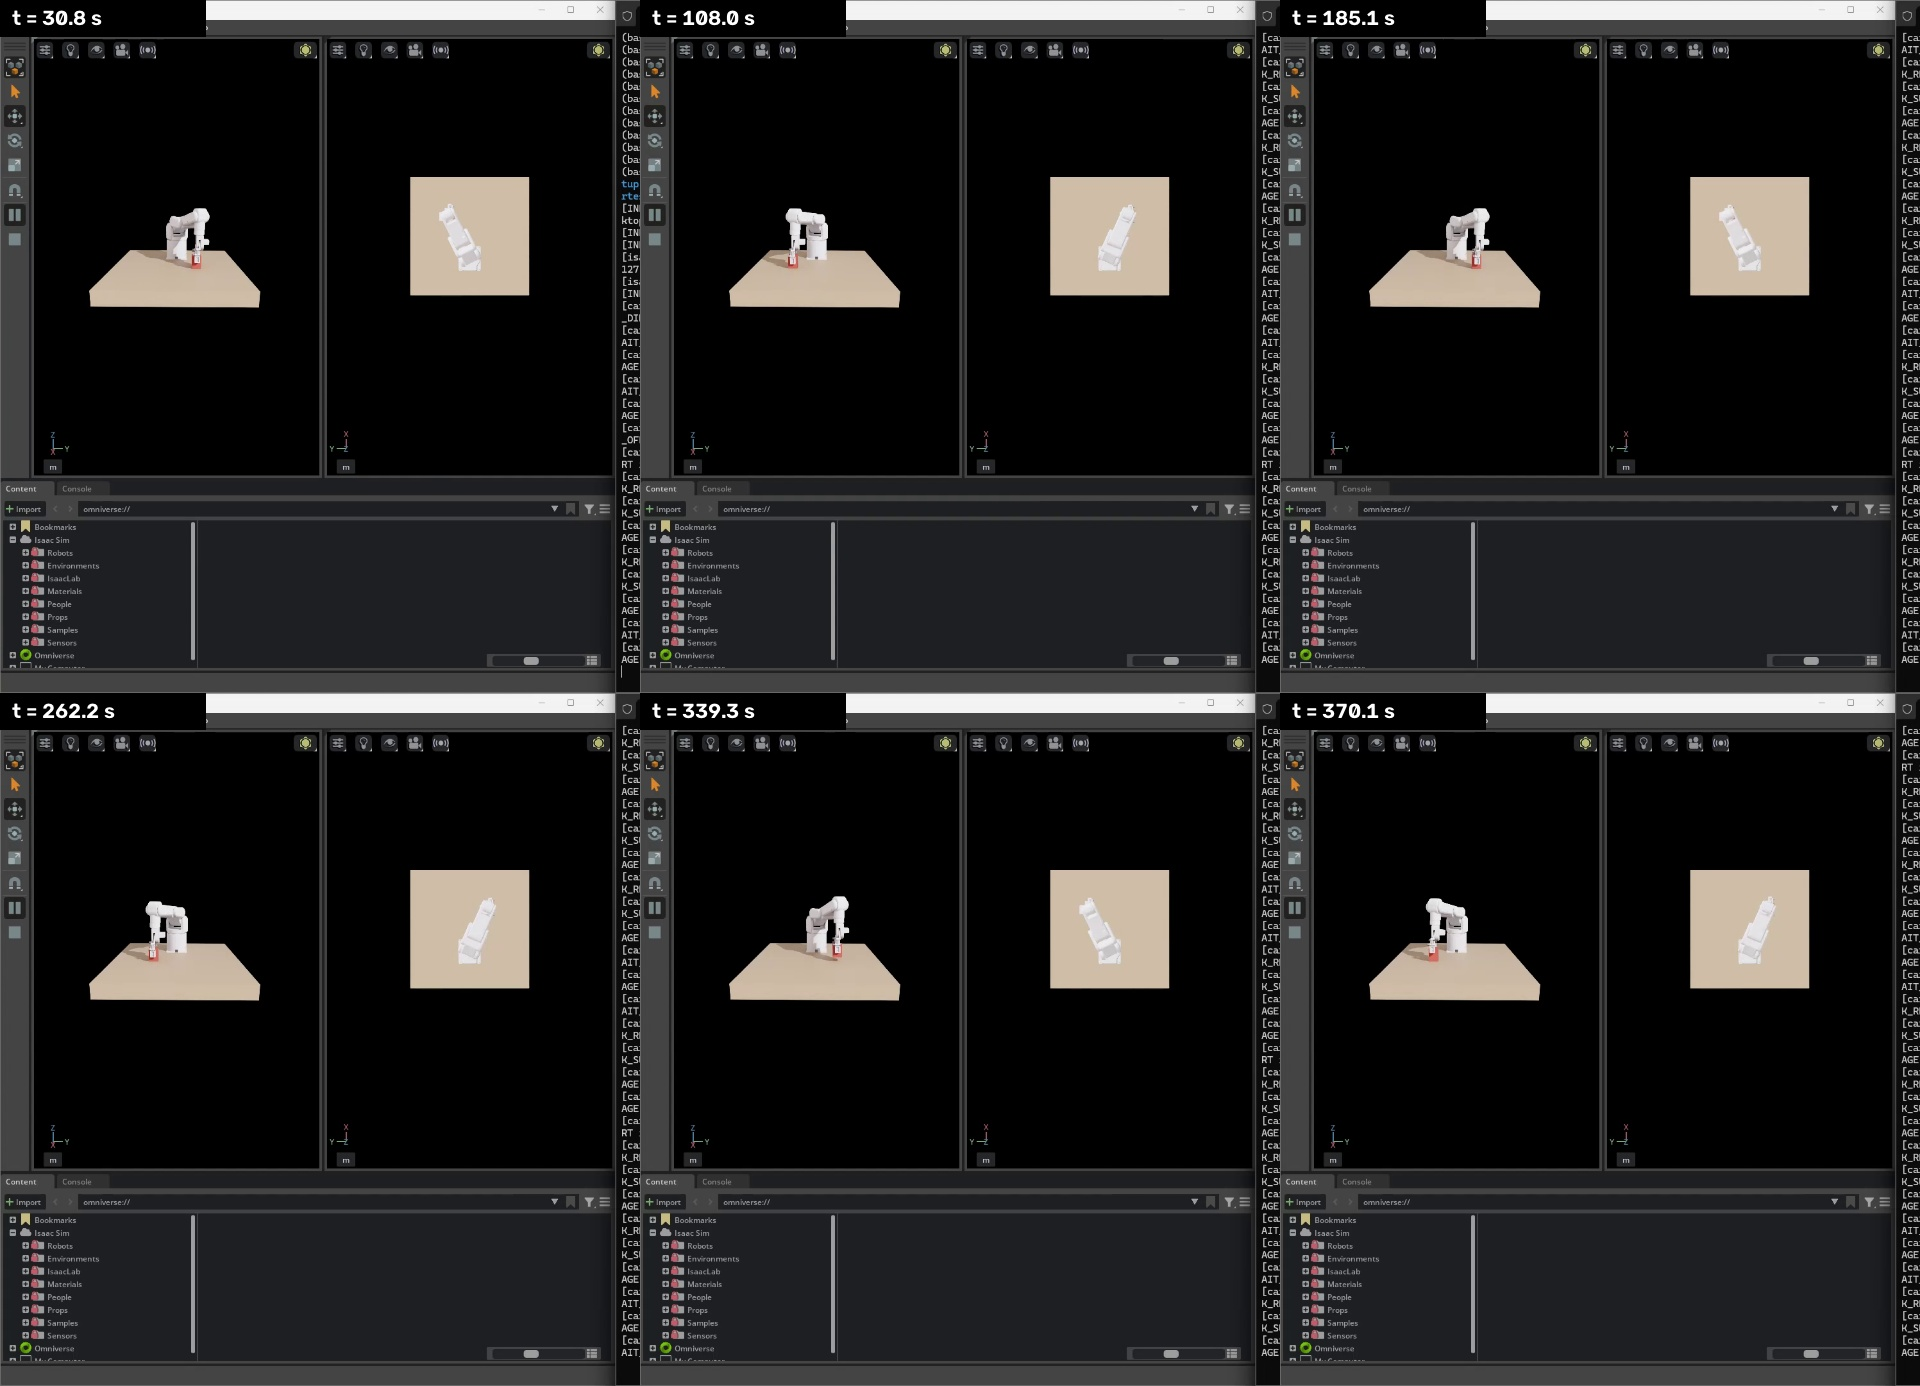
\includegraphics[width=.97\textwidth]{simulation_five_cycle_contact_sheet.jpg}
\caption{Representative frames from my completed five-cycle Isaac Sim recording}
\label{fig:simfive}
\end{figure}

The successful simulation recording is 385.57 s at approximately 30 FPS. It shows the complete alternating sequence with the scene and terminal visible. I also preserved a failed simulation attempt rather than deleting it, because failure evidence is valuable for explaining safe behavior.

\subsection{Empty-Grasp and Object Retention Logic}

The dedicated empty-grasp program intentionally closes the gripper at a reachable empty point. It emits
\begin{lstlisting}[caption={Expected controlled empty-grasp output}]
EMPTY_GRASP_EXCEPTION code=NO_OBJECT
EMPTY_GRASP_RETURN_HOME
\end{lstlisting}
then reopens, retreats, and returns HOME. This test verifies the exception path without requiring an IK failure.

In simulation, an object-retention monitor checks the distance between the gripper and target after closure. When the distance is within 0.08 m, it creates a fixed attachment for transport and removes it on release. I used this as a deterministic system-integration aid. It does not replace accurate finger-contact simulation, so I documented the distinction rather than presenting it as a high-fidelity force grasp.

\subsection{Physical Implementation on DJI RoboMaster EP}

For the real-robot stage, I adapted the fixed-point concept to the degrees of freedom available on the RoboMaster EP. The arm moves between a parked posture $(x,y)=(0,150)$ mm and a grasp posture $(220,0)$ mm. The chassis rotates to change the grasp/placement direction. Odd cycles use $+45^{\circ},-90^{\circ},+45^{\circ}$ and even cycles reverse all signs, so the object alternates between two fixed sides.

The physical sequence is:
\begin{enumerate}
\item park the arm and open the gripper;
\item rotate $45^{\circ}$ toward the source;
\item lower and extend the arm;
\item close the gripper and measure the time to the \texttt{closed} state;
\item if closure takes at least 1.85 s, classify it as an empty grasp, retreat, undo the first rotation, and retry;
\item otherwise, park the arm, rotate $90^{\circ}$ toward the destination, lower, release, park, and rotate back;
\item count only successful grasps until five successful cycles are complete.
\end{enumerate}

The program subscribes to gripper status at 50 Hz, uses a 5 s timeout for an unknown closure state, starts a 360p camera stream, and monitors the E key. Pressing E stops the chassis, pauses the gripper, suppresses later commands, stops the video stream, unsubscribes status, and closes the robot connection.

\begin{figure}[H]
\centering
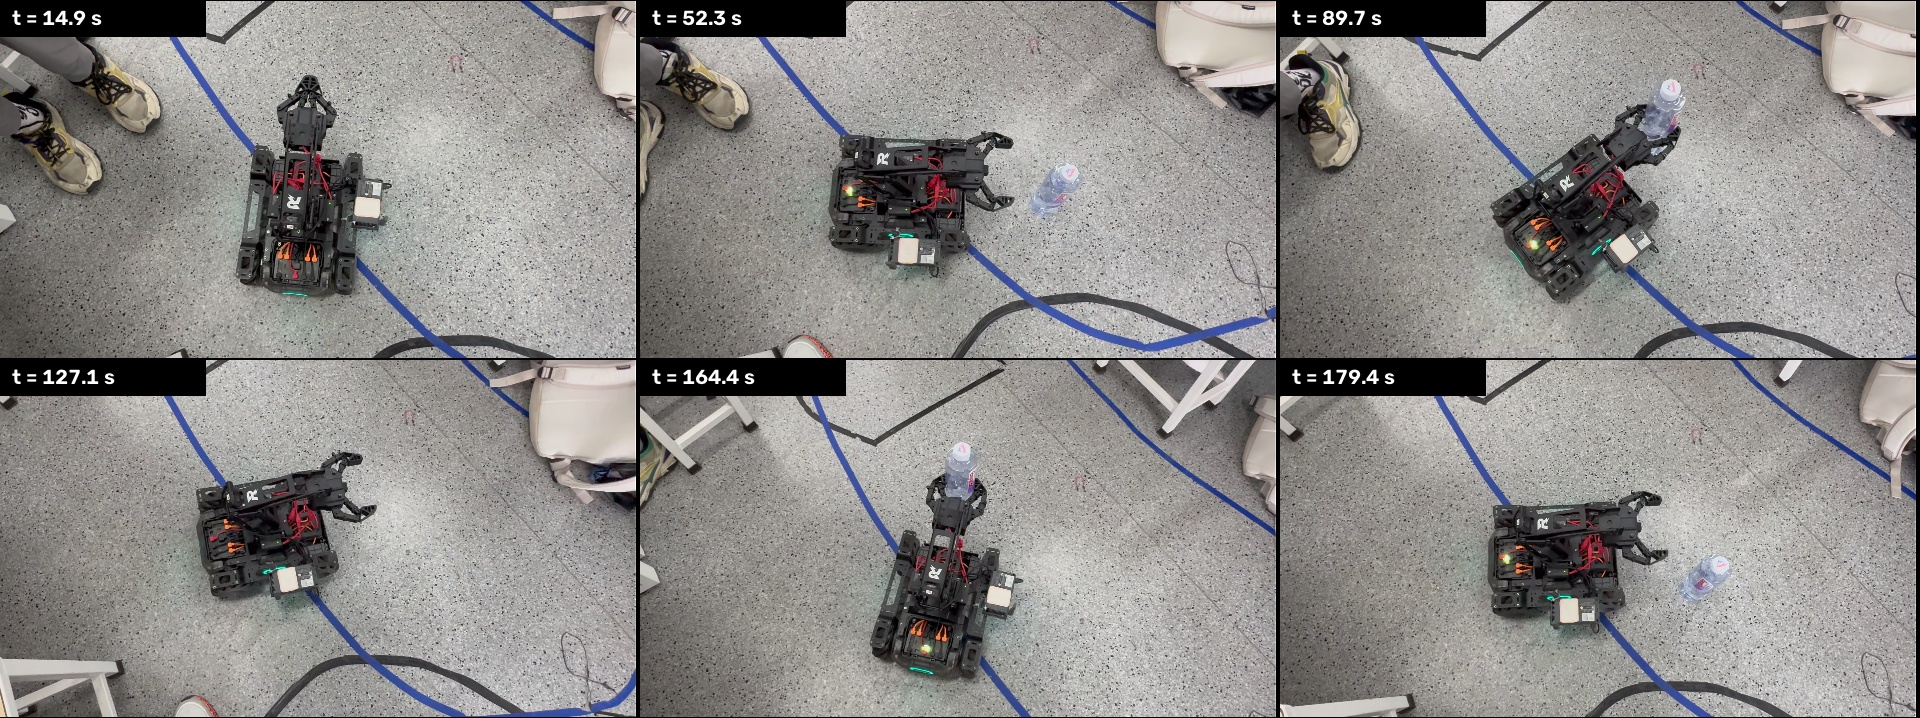
\includegraphics[width=.97\textwidth]{hardware_five_cycle_contact_sheet.jpg}
\caption{Representative frames from my completed RoboMaster EP five-cycle physical experiment}
\label{fig:hardware}
\end{figure}

The physical recording is 186.87 s at 30 FPS. It preserves real approach, grasp, chassis transfer, release, and return motion, including a failed attempt and subsequent continuation. This is important evidence that the recovery logic was exercised on the actual platform rather than described only in source code.

\section{Problems, Solutions, and Personal Reflection}

\subsection{Why I Focused on Root Causes}

The most useful lesson from this experiment was that visible robot behavior often has a cause outside the component that appears to fail. A blank RViz window may be a discovery problem, a shaking wrist may be a command-profile or drive problem, and a loose outer jaw may be a missing mechanical constraint rather than an insufficient PID gain. I therefore used a repeated method:
\begin{enumerate}
\item reduce the system to the smallest observable path;
\item distinguish command generation, transport, state feedback, and physics;
\item reproduce the symptom with a targeted probe;
\item change one layer at a time;
\item preserve both successful and failed evidence.
\end{enumerate}

\subsection{ROS 2 Discovery and Blank RViz}

\textbf{Symptom.} Isaac Sim and RViz opened, and \texttt{move\_group} printed ``You can start planning now,'' but RViz showed a Global Status warning, no \texttt{world} frame, and no initial planning scene.

\textbf{Diagnosis.} The message only proved that the local MoveIt process had initialized. It did not prove that the other ROS 2 nodes could discover it. Proxy TUN routing and mixed DDS settings caused different processes to use incompatible discovery paths.

\textbf{Solution.} I first repaired the \texttt{world -> base} static transform and RViz configuration. I then cleared stale discovery variables and tested ROS 2 communication independently. When cross-system DDS remained fragile, I moved the operational ROS graph entirely into the Docker container and used TCP only for the Windows Isaac boundary.

\textbf{Personal reflection.} I learned to treat startup messages as local evidence, not end-to-end evidence. A system is connected only when a command produces motion and the resulting measured state returns through the full path.

\subsection{Docker Build and Proxy Failures}

\textbf{Symptom.} Docker builds failed first with a non-printable session header and later while fetching the \texttt{osrf/ros:humble-desktop-full} token. A recreated container also entered a \texttt{Restarting (127)} loop.

\textbf{Diagnosis.} The project path contained Chinese characters, the Docker Desktop proxy inherited an unsuitable local proxy configuration, and an old image retained a CRLF-affected entrypoint. Recreating the container without rebuilding could not correct the image.

\textbf{Solution.} I staged the Docker build context under an ASCII-only path, configured Docker Desktop's proxy, rebuilt the image, and checked \texttt{docker compose ps} before using \texttt{exec}. I also separated image build, container startup, package build, and task launch in the documentation.

\textbf{Personal reflection.} Reproducibility depends on the host toolchain as much as on source code. I now record the exact shell, current directory, image name, and rebuild conditions instead of writing only the final ROS command.

\subsection{Motion Jerk, Shaking, and Over-Damping}

\textbf{Symptom.} Early direct targets made the arm move in steps and excite visible oscillation. Increasing damping indiscriminately removed some oscillation but made the arm slow or limp, and gripper motion could disturb the stationary wrist.

\textbf{Diagnosis.} There were three coupled causes: discontinuous target changes, target-stream timing that did not follow feedback, and gains that were not appropriate for both the arm and the gripper loop.

\textbf{Solution.} I introduced quintic 120 Hz interpolation, measured-feedback pacing, and separate normal/vertical speed limits. I then separated arm import drives from the softer gripper drives. When a dynamics change made the arm worse, I rolled it back to the last working baseline before testing another hypothesis.

\textbf{Personal reflection.} I initially treated damping as a single ``stability'' knob. The experiment showed me that stability is a property of the entire closed loop: trajectory continuity, sample timing, stiffness, damping, inertia, constraints, and collision contacts must be considered together.

\subsection{Incorrect Grasp Position and Orientation}

\textbf{Symptom.} The arm could move through the nominal sequence, but the object was not between the fingers, and the gripper was not perpendicular to the table during descent. In one later test, applying a $90^{\circ}$ yaw target caused numerical IK failure.

\textbf{Diagnosis.} A pose contains both position and orientation. Adjusting only A/B coordinates could not guarantee a vertical tool axis. Conversely, enforcing an orientation at a position near the reach boundary could make the combined target infeasible. The tool frame also differed from my initial mental model, so rotating a joint directly was not equivalent to specifying grasp yaw.

\textbf{Solution.} I derived the target orientation from the HOME tool axis, applied the $90^{\circ}$ yaw relative to that axis, and reused it throughout the grasp sequence. I added a dot-product verticality condition and adjusted the reachable pre-grasp height from 0.12 m clearance to 0.10 m. I also moved the closing point upward so the gripper surrounded the block before the palm contacted it.

\textbf{Personal reflection.} This problem changed how I think about robot poses: position and orientation must be solved together, and ``looks like a 90-degree rotation'' is not a sufficient kinematic specification.

\subsection{Missing Gripper Pins and Mimic-Joint Asymmetry}

\textbf{Symptom.} The adaptive gripper's outer links appeared loose, the distal inner and outer links were not locked together, and one side could remain stationary when the master gripper joint moved. Adding only visible pins did not repair the physical behavior.

\textbf{Diagnosis.} The visual meshes showed pivot holes, but the URDF tree omitted the two closed-loop joints. A cylinder mesh has no mechanical effect unless a constraint exists. In addition, PhysX 5.1 mimic behavior was unreliable when several follower joints shared one reference.

\textbf{Solution.} I identified the pivot coordinates from the mesh geometry, created two explicit loop revolute joints, made the outer joints passive, drove the inner joints explicitly, and mirrored the command sign in software. I retained visible pins only as a visual explanation of the constraints.

\textbf{Personal reflection.} This was the clearest example of why a visually complete CAD model is not automatically a physically complete simulation model. I had to reason from the real mechanism's degrees of freedom and constraint topology.

\subsection{Failed Attempts as Engineering Evidence}

\begin{figure}[H]
\centering
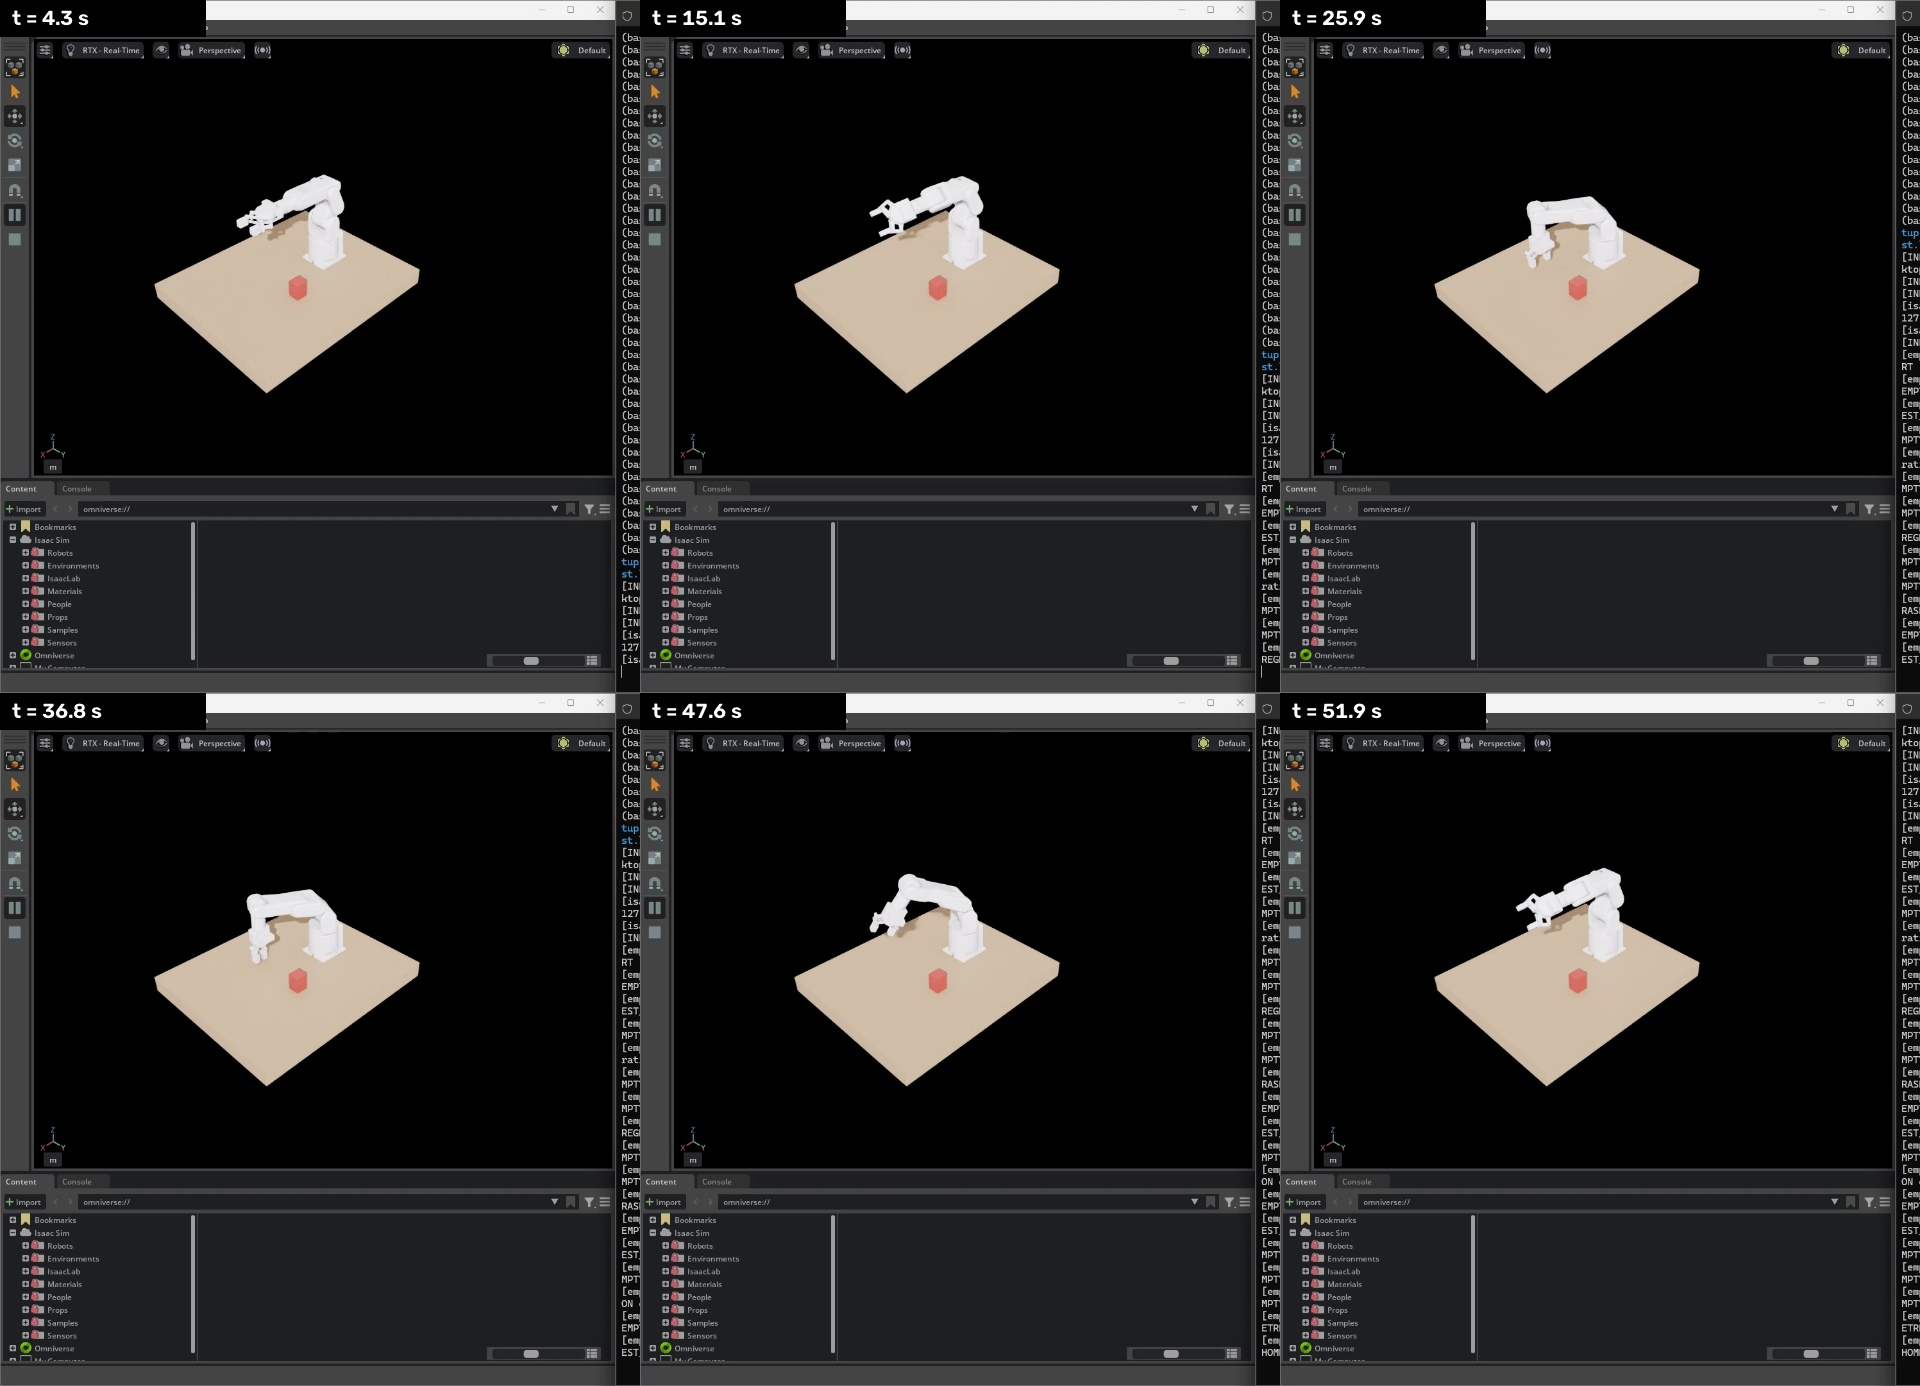
\includegraphics[width=.97\textwidth]{simulation_failure_contact_sheet.jpg}
\caption{Preserved simulation failure case used to verify visibility and bounded recovery}
\label{fig:simfail}
\end{figure}

I preserved the failed simulation recording and implemented an explicit empty-grasp test because a successful video alone cannot demonstrate safe exception behavior. On the physical robot, I used gripper closure time as an available heuristic: a quick \texttt{closed} signal indicates an object obstructed full closure, while a long closure indicates an empty grasp. This is not a calibrated force sensor, but it is a practical observable signal for the available hardware.

The physical program distinguishes three cases:
\begin{itemize}
\item closure below 1.85 s: count the grasp and transfer;
\item closure at or above 1.85 s: classify as empty, retreat, and retry without increasing the success count;
\item no closed state within 5 s: preserve the current state and enter safe exit because the result is unknown.
\end{itemize}
My main lesson was to represent uncertainty explicitly. A timeout should not be silently converted into success or failure.

\subsection{Summary of Major Problems and Decisions}

\begingroup\small
\begin{longtable}{p{2.8cm}p{3.3cm}p{4.1cm}p{2.6cm}}
\caption{Problem-solving summary}\label{tab:problems}\\
\toprule Symptom & Root cause & Final decision & What I learned\\
\midrule\endfirsthead
\toprule Symptom & Root cause & Final decision & What I learned\\
\midrule\endhead
RViz blank/global warning & DDS discovery and missing fixed frame & Container-local ROS graph, static TF, TCP Isaac boundary & Verify the full data path\\
Docker build timeout/error & Proxy, Unicode path, stale CRLF image & ASCII staging, proxy correction, clean image rebuild & Host setup is part of reproducibility\\
Stepped and shaking motion & Target discontinuity and timing/gain mismatch & Quintic interpolation, 120 Hz streaming, feedback pacing & Smooth commands before tuning gains\\
Slow vertical contact needed & One speed for all stages & 28 deg/s transit and 4 deg/s vertical stages & Motion context should select speed\\
Palm hit before closure & Closing target too low & Dedicated 0.04 m closing clearance & Model the object top, not only its center\\
IK failed after yaw change & Combined pose near reach boundary & HOME-relative yaw, vertical metric, reachable clearance & Position and orientation are coupled\\
Outer gripper links loose & Missing closed-loop constraints & Two distal loop revolute joints & Mesh appearance is not physics\\
One gripper side unresponsive & Multiple-follower mimic limitation & Disable mimic parsing and mirror explicit drives & Middleware/model shortcuts need validation\\
Empty grasp counted as success & No grasp-result observation & Closure-time heuristic, retry, unknown-state timeout & Uncertainty needs a separate state\\
\bottomrule
\end{longtable}
\endgroup

\subsection{Personal Growth}

This project developed four habits that I consider more valuable than any single parameter value.

First, I learned to build a narrow diagnostic probe before debugging the complete task. The \texttt{direct\_motion\_probe} proved outbound motion and return feedback independently of MoveIt planning. That reduced a complicated integration failure to a transport/control question.

Second, I learned to separate model geometry from physical semantics. Repairing the gripper required locating the correct bodies, local pivot coordinates, joint axes, drive ownership, and collision behavior. It was not enough to add a visible bolt.

Third, I learned to preserve traceability. Small commits, explicit logs, failure recordings, and parameter files made it possible to explain why the final system works and to recover when a tuning change made it worse.

Finally, I learned to adapt one task principle across different robots. The simulated mechArm and physical RoboMaster EP do not share the same kinematics, but both implement fixed source/destination locations, a safe posture, controlled approach, grasp feedback, transport, release, repetition, and recovery. That abstraction is what made the experiment transferable.

\section{Conclusion}

I completed both parts of Experiment 2 with the equipment available to me: a mechArm 270 Pi adaptive-gripper simulation in Isaac Sim and a physical DJI RoboMaster EP experiment. The simulation executes vertical fixed-point grasping, five alternating transfers, and controlled exceptions through a Dockerized ROS 2/TCP architecture. The physical program completes five successful grasp-and-place cycles while monitoring the gripper, retrying empty grasps, displaying the camera, and providing a safe-exit path.

My main contribution was not a single script but the integration of model, physics, kinematics, transport, feedback, real hardware, evidence, and documentation. The public repository history, simulation recordings, failure recording, physical recording, and source cross-reference provide a verifiable account of that work. The project also taught me to distinguish visible symptoms from root causes and to treat failed attempts as useful engineering evidence.

\appendix

\section{Repository Evidence Cross-Reference}

\begin{longtable}{p{4.2cm}p{8.7cm}}
\caption{Evidence and implementation paths}\\
\toprule Evidence topic & Repository path\\
\midrule\endfirsthead
\toprule Evidence topic & Repository path\\
\midrule\endhead
Simulation startup and scene & \path{scripts/start_isaac.ps1}, \path{simulation/isaac/start_simulation.py}, \path{simulation/scenes/mecharm_pick_place.usd}\\
Official model assets & \path{simulation/urdf/mycobot_description/}\\
Cartesian task parameters & \path{src/mecharm_pick_place/config/direct_cartesian_pick_place.yaml}\\
Numerical IK & \path{src/mecharm_pick_place/mecharm_pick_place/numeric_ik.py}\\
Smooth execution & \path{src/mecharm_pick_place/mecharm_pick_place/direct_pick_place_demo.py}\\
Five-cycle task & \path{src/mecharm_pick_place/mecharm_pick_place/cartesian_direct_pick_place.py}\\
Five-cycle launch & \path{src/mecharm_pick_place/launch/alternating_cartesian_pick_place.launch.py}\\
Empty-grasp exception & \path{src/mecharm_pick_place/mecharm_pick_place/empty_grasp_test.py}\\
TCP transport & \path{simulation/isaac/tcp_joint_bridge.py}, \path{src/mecharm_pick_place/mecharm_pick_place/tcp_bridge_node.py}\\
Adaptive-gripper repair & \path{simulation/isaac/start_simulation.py}\\
Object retention & \path{simulation/isaac/grasp_monitor.py}\\
RoboMaster EP five-cycle retry & \path{robomaster_ep/scripts/pick_rotate_place_5_cycles_retry.py}\\
Simulation/physical recordings & \path{docs/videos/}\\
Operating instructions & \path{README.md}, \path{README_EN.md}, \path{robomaster_ep/README.md}\\
Public commit evidence & \path{report/individual_report/evidence/git_history.txt} and Figure~\ref{fig:github}\\
\bottomrule
\end{longtable}

\section{Reproducible Operating Commands}

\subsection{Simulation Startup}

From Windows PowerShell, after changing to the Experiment 2 project root:
\begin{lstlisting}[caption={Start Docker runtime and Isaac Sim}]
.\scripts\start_moveit_sim.ps1
\end{lstlisting}
After the container is running, the ROS 2 workspace build command is:
\begin{lstlisting}[caption={Build the ROS 2 packages inside Docker}]
docker compose exec moveit bash -lc \
 "source /opt/ros/humble/setup.bash && \
  colcon --log-base /opt/mecharm_ws/log build \
  --base-paths /workspace/mecharm_exp2/simulation/urdf/mycobot_description \
  /workspace/mecharm_exp2/src \
  --build-base /opt/mecharm_ws/build \
  --install-base /opt/mecharm_ws/install --symlink-install"
\end{lstlisting}

The five-cycle task is launched with:
\begin{lstlisting}[caption={Execute five alternating simulation cycles}]
docker compose exec moveit bash -lc \
 "source /opt/ros/humble/setup.bash && \
  source /opt/mecharm_ws/install/setup.bash && \
  ros2 launch mecharm_pick_place \
  alternating_cartesian_pick_place.launch.py \
  project_root:=/workspace/mecharm_exp2 cycles:=5"
\end{lstlisting}

\subsection{Physical-Robot Startup}

After connecting the computer to the RoboMaster EP Wi-Fi and clearing the work area:
\begin{lstlisting}[caption={Run the physical five-cycle retry program}]
conda activate robomaster
$env:RM_SDK_ROOT = "C:\Users\xhr\RoboMaster-SDK-fixed"
python robomaster_ep\scripts\pick_rotate_place_5_cycles_retry.py
\end{lstlisting}
The operator presses Enter to begin and can press E at any time to request safe exit.

\section{Evidence Integrity Note}

The GitHub screenshot was captured directly from the public \texttt{main} commit page. The 31 pushed commits and their author are also stored as plain-text evidence. The contact sheets were sampled programmatically from the original MP4 recordings without changing the source videos. Their measured metadata is:
\begin{table}[H]
\centering
\caption{Recorded experiment evidence}
\begin{tabularx}{\textwidth}{Yrrr}
\toprule Recording & Duration (s) & FPS & Frames\\
\midrule
Successful five-cycle simulation & 385.57 & 30.002 & 11,568\\
Preserved simulation failure & 54.06 & 30.004 & 1,622\\
RoboMaster EP five-cycle physical run & 186.87 & 30.000 & 5,606\\
\bottomrule
\end{tabularx}
\end{table}

The ROS 2 workspace build previously completed four packages in 11.6 s. A lightweight source/configuration test run produced 36 passes and two failures. The two failures were stale contract assertions: one expected an older initial gripper-close sequence, and the other expected an earlier $8^{\circ}/\mathrm{s}$ vertical speed while the implemented value was $4^{\circ}/\mathrm{s}$. I report these results because transparent evidence is more useful than presenting an artificial all-green test result.

\begingroup\small\linespread{1.0}\selectfont
\begin{thebibliography}{9}
\bibitem{guide} Robotics Systems Integration Laboratory. \emph{Mechanical Arm Fixed-Point Grasping Experiment Requirements}, 2026.
\bibitem{elephantrepo} Elephant Robotics. \emph{mycobot\_ros2: myCobot ROS 2 Package, Humble Branch}. \url{https://github.com/elephantrobotics/mycobot_ros2}.
\bibitem{isaac} NVIDIA Corporation. \emph{Isaac Sim Documentation, Version 5.1.0}. \url{https://docs.isaacsim.omniverse.nvidia.com/5.1.0/}.
\bibitem{ros2} Open Robotics. \emph{ROS 2 Humble Documentation}. \url{https://docs.ros.org/en/humble/}.
\bibitem{moveit} PickNik Robotics. \emph{MoveIt 2 Documentation: Humble}. \url{https://moveit.picknik.ai/humble/}.
\bibitem{robomaster} DJI. \emph{RoboMaster Python SDK Documentation}. \url{https://robomaster-dev.readthedocs.io/}.
\end{thebibliography}
\endgroup

\end{document}
